\section{Problem Description}
Since this project is focussed on extractive summarization, the aim is to select sentences from the source article that could be considered worthy of being included in the summary.
So I decided to approach this as a problem of classification of sentences (in the source document) into one of the two classes: 'belonging' to summary and 'not belonging' to summary.

\section{Data Collection}
Collecting a standard dataset for this task was not easy.
There are no publicly available datasets consisting of scientific articles and their respective summaries.
Hence, in order to build a dataset, articles were randomly sampled from the ACL Anthology.
For the initial phase, 11 scientific articles were sampled to make up a small dataset to run the baseline on.
This set of articles will be referred to as Data Set 1 in this report.
For the second phase, 20 more articles from the same database were sampled.
This set will be referred to as Data Set 2.
Since the second phase involved experimentation with classificaiton algorithms, this set of 20 documents (Data Set 2) was used for training and the set of 10 documents (Data Set 1) that was sampled earlier was used as the test set.

\section{Evaluation Criteria}
In accordance with the aim of the project, the evaluation of any system built should be based on the quality of summary produced by that system.
Another constraint that was considered for this project was the length of the summary.
It was decided that a summary should not exceed the length of 100 words.
Being extractive in nature, the limit is imposed after discounting the stop words in the sentences.

For a quantitative judgment, the performance of both the baseline and further development over baseline is measured using ROUGE scores.
ROUGE [...] is an summary evaluation system that measures the similarity of an automated summary with a set of reference summaries.
Each automated summary can be evaluated against multiple reference summaries of the same text to get a better judgement about the automated summary.

For this project, a gold standard set was created to be used as reference summaries.
The gold standard consisted of multiple summaries for each of the articles in Data Set 1.
For each article, sentences that seemed most suitable for the summary of that article (based on human annotator judgement) were manually extracted untill the aforementioned word limit was reached.
This was done for each article in Data Set 1 by each annotator.
The annotators consisted of all the members of the group that I worked with for this project.

In the second phase of the project, experiments done involved the classification of individual sentences into one of the two classes mentioned above.
For this purpose, I extracted a set of sentences from each of the articles in Data Set 1.
Then, I manually labelled these sentences into one of the two classes: 0, meaning the sentence is not suitable to be included in the ideal summary; or 1, meaning the sentence can be included in the ideal summary.
The performance of using different features for classification of individual sentences was evaluated based on this labelled set of sentences.

\section{Pre-Processing}

\section{Baseline}
The first step was to build a basic system that could be the basline for further experiments and improvements.
Another factor for consideration was that the aim of the project was to create an extractive summary consisting of sentences from the same document that needs to be summarized.
After studying various approaches used by researchers for single document summarization, I decided to use an unsupervised ranking algorithm.
Following is a brief description of the TextRank algorithm, as introduced by \citep{Mihalcea et. al.[]}, to explain how a graph based raking algorithm can be applied to rank sentences within a document.

\subsection{TextRank}
The basic idea implemented by a graph-based ranking model is that of 'voting' or 'recommendation'.
When one vertex links to another one, it is basically casting a vote for the other vertex.
The importance of a vertex is based on the number of votes casted towards that vertex. 

Formally, let \emph{G = (V, E)} be a directed graph with the set of vertices \emph{V} and set of edges \emph{E} where is a subset of \emph{{V x V}}.
For a given vertex \(V_i\), let \(In(V_i)\) be the set of vertices that point to it, and let \(Out(V_i)\) be the set of vertices that \(V_i\) points to.
The score of vertex \(V_i\) is defined as follows (\emph{Brin and Page []}),
\[S(V_i) = (1 - d) + d * \sum_{j \in In(V_i)} \frac{1}{|Out(V_j)|}S(V_j)\]
where \emph{d} is the damping factor that can be set between 0 and 1.
The factor \emph{d} is generally set to \emph{0.85} and this the value that was used for my experiments as well.
Starting with arbitrary values assigned to each node in the graph, the computation iterates untill convergence below a given threshold is achieved.
The final score associated with each vertex represents the \textit{importance} of that vertex within the graph.

Two modifications were introduced by \emph{Mihalcea []} to apply this algorithm to documents for ranking sentences.
The first modification was to define the above mentioned algorithm for undirected graphs in which case, the out-degree of the vertex is equal to the in-degree of the vertex.
The other modification was to incorporate the notion of \textit{strength} of the connection between any two vertices as a weight \(w_ij\) added to the corresponding edge that connects the two vertices.
Consequently, the new formula that takes into account these two modifications and gives the weighted score is
\[WS(V_i) = (1 - d) + d * \sum_{V_j \in In(V_i)} \frac{w_ji}{\sum_{V_k \in Out(V_j)}w_jk}WS(V_j)\]

\subsection{TextRank for Summarization}
To apply this algorithm for ranking sentences, a graph a built in which the sentences (from the source document) represent the vertices of the graph, and the edges between these vertices is defined by the sentence 'similarity'.
Here, 'similarity' is a measure of the content overlap between the two sentences that connected by that edge.
This overlap of content between any two sentences can be defined by the number of common tokens between the lexical representations of the two sentences.

For the purpose of the work described in thesis, this concept of similarity between sentences within a document has been implemented in the following way.
A matrix of \emph{tf-isf} (term frequency - inverse sentence frequency) is contructed for the entire document.
This tf-isf matrix is then multiplied by its transpose to obtain the similarity matrix with dimensions equal to the number of sentences in the entire document, and each value representing the similarity between the two sentences used to index that value in the matrix.

After running the ranking algorithm over this graph untill convergence, the sentences are sorted in decreasing order based on the final score.
The top ranked sentences are selected for inclusion in the summary.
The performance of this algorithm on scientific articles as baseline is documented in detail in the Experiments and Results section of this report.
This is chosen as the baseline as it has been shown to perform reasonably well on unstructured text, for example news articles.

Considering that the corpus used for this project consists of scientific articles from the ACL Anthology, these articles are generally about a specific study and elaborate on the methodology of the conducted experiments, the results obtained, conlusion and possible discussion arising from conducting the experiments.
These also include an "Introduction" section as well as a "Related Work" section to describe the work of others who have addressed the same or similar problem.
The performance of the baseline has been documented in Section 4.

Although the performance of the baseline system was decent, further qualitative analysis of the summaries generated by this baseline showed that these summaries included sentences which varied in degree of suitability to be included in the ideal summary.
Here ideal summary would be one that is similar in content to the summary created by humans as in the gold standard that is used in this project.
Each of the extracted sentence from this baseline was objectively judged as to whether its contents were important enough for that sentence to be included in the ideal summary.
It was found that 30\% of all the extracted sentences were not suitable in this respect.

\todo{Add example from baseline and also stats above if possible,  ROUGE paper}

The evaluation of baseline helped in understanding that it is not enough to rely on an algorithm that ranks sentences based on content overlap with other sentences.
The importance of the words within the sentence should also be considered.
I decided to explore how the importance of words appearing in a sentence, with respect to the article being summarized, relates to whether that sentence should be included in the summary or not.
It is also important to limit the examination to words that contribute to the immediate (central) meaning conveyed by the sentence as opposed to considering adjunct clauses or phrases that do not contribute much to the central meaining of the sentnece.
The following sections, I have doumented the different experiments tried out to this end.

\section{Data Preparation}
Before explaining the different experiments tried, I would like to explain the preparation of training and test sets for the second phase of the project.
As mentioned earlier, data colleciton was a difficult process as there is no publicly available data for such a task.
In Section 3.2, I have mentioned that two data sets were prepared, Data Set 1 and Data Set 2.
Scientific articles in Data Set 1 were used in the first phase (described above) to extract sentences to form summaries and then the ROUGE score of the baseline summarizer was calculated by comparing the generated summaries against the gold standard summaries.

In Section 3.3, I have mentioned that articles in Data Set 1 were further processed to get labelled sentences.
This was done in the following manner.
For each article in Data Set 1, all the sentences were ranked using TextRank and the top 7 sentences were chosen.
These 7 sentences were manually labelled as belonging to either class 0 or class 1.
The rationale behind using TextRank for such sampling is that this ranking algorithm is the baseline.
Being the baseline, it will be used in the pipeline of the final system after the preprocessing step.
So the input to the classification algorithm would come from this baseline module.
Hence, to create a test set of labelled sentences to evaluate the performance of the classification module, I decided to use the top 7 seven sentences ranked by the baseline, from each of the article in Data Set 1.
Since Data Set 1 consisted of 11 articles, there were 77 labelled samples in the test set of which 33 were positive and 44 were negative samples.

For the training set, Data Set 2 was used, which consisted of 20 articles.
Since it is not easy to manually label sentences in each document into the desired classes, I applied an approximation.
This is based on the fact that the abstract of a scientific article represents the information that has to be included in the summary.
So I decided to consider all the sentences in the abstracts of all the articles in Data Set 2 to be positive samples for classification.

For negative sample collection, for each article in Data Set 2, I ranked all the sentences using TextRank and chose the lowest ranked sentences.
I made the assumption that if a sentence is ranked low by TextRank, then it is not suitable to be included in the summary and can be considered a negative sample.
In the previous section, I argued that a high degree of content overlap of a sentence with other sentences in the document is not definitively indicative of its importance with respect to the document.
However, if this degree of content overlap is very low, it indicates that the content in that sentence is either too specific to have appeared often in the document, or the content is irrelevant with respect to the main topic of the entire document.
In either case, such a sentence can be considered as a negative sample.
There were 183 samples in the training set of which 83 samples were positive and 100 were negative.
A small point to be noted is that while sampling these negative sentences, I eliminated setences which can not be considered valid sentneces. This validity is defined by sentence length(between 15 to 40 words was considered valid) and presence of non-alphanumeric characters.

\section{Dependency Parses}
A dependency parse of a sentence represents the grammatical relationships of words in that sentence.
It is different from a constituent parse of a sentence.
While a constituent parse breaks a sentences into different phrases down to the individual words (commonly known as phrase structure representation), a dependency parse is used to represent the textual relationships between words in that sentence.
Depending on the language as well as the purpose of the analysis, different dependency grammer conventions can be used.

For this project, I decided to follow Stanford Typed Dependency [...] relations.
In this kind of dependency parse, each word is associated with another word and this association is defined by a dependency relation.
There are around 50 grammatical relations (dependencies) defined for Stanford Type Dependency Parser.
Consider the following example:

\emph{Bills on ports and immigration were submitted by Senator Brownback, Republican of Kansas}

For the above sentence, the Stanford Types Dependencies as well as a graphical representation of this dependency parse is shown in Figure 3.1.

\begin{figure}[h]
\begin{subfigure}{0.5\textwidth}
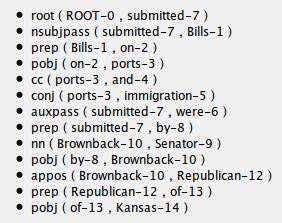
\includegraphics[width=0.9\linewidth, height=5cm]{typed_dependencies1} 
\caption{Stanford Typed Dependencies}
\label{fig:typed-dep}
\end{subfigure}
\begin{subfigure}{0.5\textwidth}
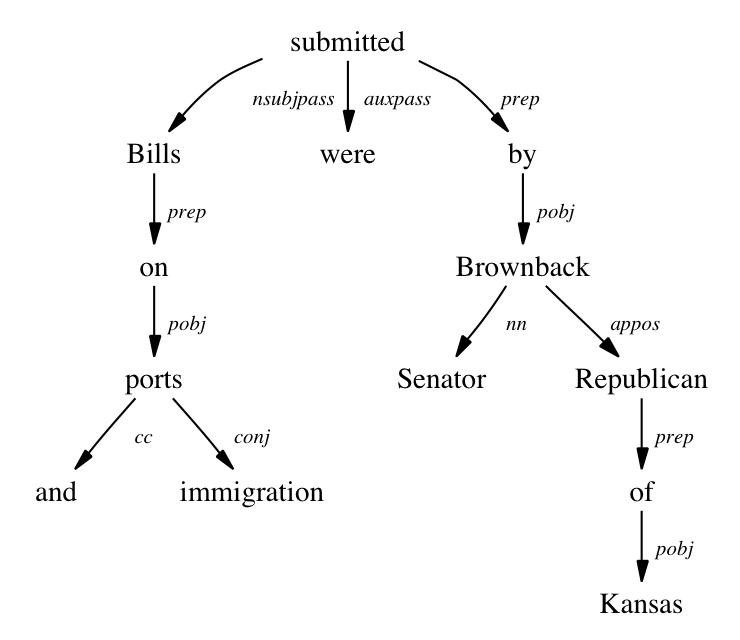
\includegraphics[width=0.9\linewidth, height=5cm]{typed_dependencies2}
\caption{Dependency Parse graph}
\label{fig:dep-parse}
\end{subfigure}
 
\caption{Stanford Dependency Parse}
\label{fig:stanford-dep-parse}
\end{figure}

It can be seen that this kind of dependency parse helps in identifying the latent relationships between different words in a sentence.

As described in the previous section, the baseline uses the textual content overlap of a sentence with others in the document to decide how important the sentence within that document.
The baseline algorithm does have the ability to process information beyond the textual content in a sentence.
Therefore, I decided to use dependency parse of sentences to extract information that could be used as features to classify each sentence into one of the classes defined earlier (0 or 1).

In the folowing sections, I describe my experiments in extracting useful features from dependency parse trees for this purpose.

\section{Convolution Kernels}
Kernel methods are one of the popular pattern recognition algorithms that use kernel functions to map high dimensional data points to an inner product space in order to apply linear classification in this new space.
Support Vector Machines[...] is a well know kernel method that is used for pattern classification classification.
Depending on the nature of data, SVM can be used with different types of kernels such as linear, polinomial, radial basis function and many others.
For example, with numerical data, using a liner kernel will map high dimansional data points into a feature space, where only the distance between the projections of data points over a certain line (defined by the kernel) will be used for drawing margins for classification.

In this report, I discuss the use of Convolution kernel \citep{Collins and Duffy []}, which is a type of string kernel that makes use of the structural information within a sentence.
Convolution kernels use the sentence tree structures and calculate the similarity between two trees.
This is done by recursively counting the number of identical sub-trees that appear in both input trees.

\todo{Convolution kernel equation}

Hence, convolution kernles can help in providing a mapping between the sentences and their structural similarity with other sentences.

\citep{Moschitti et. al.[]} describe an efficient algorithm for using convolution kernel as the kernel function for SVM.
They have used the SVM-light library and included a new kernel definition for efficient computation of convolution kernel \citep{SVM-light-TK []}.
This library can take any kind of parse tree as input.

\subsection{Experiment}
I decided to use SVM-light-TK for classification of sentences.
Each sentence was first passed through the Stanford Parser and the dependency parse tree for the sentence was obtained.
Each node in the parse tree consisted of 3 components : the actual word on that node, the part of speech tag of that word and its dependency relation with its parent node.
This representation for the following sentence has been shown in Figure 3.2.

\emph{The user could ask it to build up a computer configuration satisfying his particular needs.}

\begin{figure}[h]
\centering
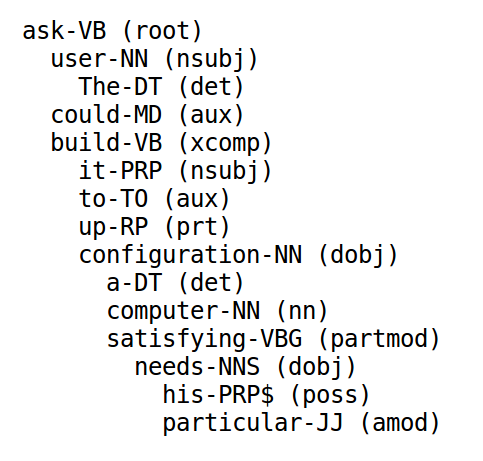
\includegraphics[width=0.4\linewidth, height=5cm]{typed_dependencies3} 
\caption{Dependency Parse representation from Stanford Parser}
\label{fig:dep-parse}
\end{figure}

SVM-light-TK has the provision of specifying more than one tree structure as the feature vector for each sentence (sample).
So, I separated each component of each node and created feature vector containing three trees.
The first tree consisted of the words.
The second tree consisted of the nodes in the same position, but only the part of speech tags of the words were used.
Similarly, the third tree contained only the dependency reations of each node to its parent.

The classification was done over the training set and the model was tested over the test set as mentioned in the section on Data Preparation.

\subsection{Results}
Following is the result of using convolution kernels to train SVM over the training sentences.
The confusion matrix of the model tested over the test set is shown in Table ...

It can be seen that the values of both Precision and Recall of the model over the test set are very low.

\subsection{Discussion}
The poor performance of the classifier using convolution kernel can be explained by considering the inherent nature of convolution kernels.
Convolution kernels are used to classify sentences on the basis of structural differences (or similarities).
As explained earlier, they work on the principle of finding similar structures of sub-trees between two trees.
However, for the task at hand, sentences have to be classified on the basis of how similar the content is to the main topic being discussed in the article.
In that respect, the structure of a sentence and the variability in the dependency relations of words within that sentence do not provide any indication about the importance of the content in that sentence.

The above experiment and analysis helped in the realization that for classificaiton of sentences into the desired classes, the content of a sentence has to be examined closely for better feature extraction.

\section{Importance Features}
I decided to concentrate on the different parts of a dependency tree.
There are three important grammatical componenets in a dependency parse of a sentence that I decided to look into : \textit{verb, subject} and \textit{object}.
It can be seen from the dependency parse representation that the main \textit{verb} in the sentence is the \textit{root} of the parse.
In accordance with the rules of English grammar, the main verb is associated with either a subject or an object or both a subject and an object.
This can be noticed in the dependency parse as well.
Consider the dependency parse shown in Figure 3.2.
The subject in the sentence is 'user' and its dependency relation to the main verb 'ask' is 'nsubj' which means \textit{nominal subject}.
Similarly, there is an object in the sentence, 'configuration' which is related the verb 'build' (which is not the main verb in the sentence) by the relation 'dobj' which means \textit{direct object}.

It was my hypothesis that these three dependency relations can be helpful in identifying phrases containing words that should be examined for importance.
By importance, I mean the degree of closeness of these words to the main topic of discussion in an article.
This importance can be measured using various text-based metrics using in Information Retrieval and Text Processing such as the total count of occurance of words, their term frequency inverse document frequency (tf-idf) and term frequency inverse sentence frequency (tf-isf).

Stanford Typed Dependencies [...] define the relation between a verb and the subject attached to it using different dependency relations depending on the context. These are \textit{csubj, csubjpass, nsubj, nsubjpass} and \textit{xsubj}.
Similarly, the dependency relation between a verb and the attached object is defined by \textit{dobj, iobj} and \textit{pobj}.
For this experiment, I did not consider the different types of subject and object dependencies as I was only interested in finding the subjects and objects irrespective of the context with the verb.

\subsection{Experiment}
For each sentence, its dependency parse tree is first obtained.
Since the verb is the root of the tree, it can be easily accessed.
The algorithm then searches for both subject (the letters 'subj' in the dependency relation) and object (the letters 'obj') in the dependency tree.
The search for subject and object in the tree is Breadth-First Search in order to find the subject and object as high up in the tree as possible.
This is done because a sentence might contain multiple subjects or objects.
In such a case, it is important to pick up the subject (or object) that is closer to the main verb of the sentence.
After obtaining these three nodes, verb, subject and object, the importance of these nodes is to be calculated using the metrics mentioned above.

For the subject node, all the nodes in the sub-tree with the subject as the root are also considered for the calculation of importance.
The same is true for the object node as well.
This is done because I wanted to capture the importance of the entire phrase associated with the subject and the object.

\subsubsection*{Metrics}
For this task, the corpus consists of documents that have to be individually summarized.
This means that the system obtained from this effort needs to take a single document as input and produce its summary without the context of any other document.
The purpose of using a corpus of documents for this task is to collect statistics over multiple documents rather than treating the corpus as a controlled set.
Hence, I decided to exclude the computation of term frequency inverse document frequency (tf-idf) of words within a document with respect to the entire corpus.

The metrics that I used in experiments for the computation of 'importance' of verb, subject phrase and object phrase in each sentence are : \textit{count}, \textit{trem frequency inverse sentence frequency (tf-isf)}, and \textit{term frequency inverse section frequency (sec-tf-idf)}.

Count represents the count of the word being considered throughout the entire document.
The tf-isf is calculated in the same way as term frequency inverse document frequency is calcualted. The only difference is that for tf-isf, the sentence containing that word is considered the 'document' and the entire article (document containing the sentence) is treated as the corpus.
The sec-tf-idf is also calculated in a similar way as tf-idf.
Except that in this case, the section in which that word occurs is treated as the 'document' and the entire article is treated as the corpus.
The information about the section is obtained from the preprocessing step from the annotations of the output from the software package ParsCit/SectLabel [...].

\subsubsection*{Feature Extraction}
For the verb node, the calculation of the features is straight-forward.
The three metrics are obtained for the word representing the verb node.
For subject phrase, the tf-isf of each word (node) in the subtree (with the subject node as the root) is calculated.
If the word is a stop-word, then the tf-isf value for that node is assigned as 0.
Once the tf-isf values of all the words in the subject phrase have been obtained, the average of these values is computed.
This average value is used as the tf-isf value of the subject phrase.
The values of count and sec-tf-idf are also calculated in the same way.
Also, the same process is followed for calculating these metrics for the object phrase.

\todo{missing values}

A point to be noted is that the list of stop-words was modified.
All first-person and third-person pronuouns were removed from the stop-word list.
The reason behind this is that, considering the domain of the task, it is common to find sentences in scientific articles that contain the word 'we'.
Such sentences generally decribe the work done by the authors of the article and most probably the work done in the same study that the article is about.
Likewise, it is common to find sentences that contain the word 'they' and such sentences generally point to work done by other researchers that are cited by the authors of the article.
Hence, these words can not be ignored.

Once these features are obtained, the training set is used to used to train an SVM classifier with RBF kernel.
I tried different combinations of features and tuning parameters which are listed below.
\begin{itemize}
\item The count, tf-isf and sec-tf-idf features were considered separately.
\item The three metrics were considered together.
\item The \textit{gamma} value for the SVM classifier was varied from 0.001 to 100
\item For calculation of the metric over the sub-tree, for every descent to a lower level in the tree, the value of the metric at that level is multiplied to a factor.
This factor was reduced bya constant degree with each level ranging from 0.5 to 2.
This was done to reduce the effect of lower values of nodes in the sub-tree that couldbe responsible for reducing the value of the entire phrase.
\end{itemize}

Section 4 documents the results obtained from these experiments.

\section{Final Pipeline}
The final pipeline is contructed of the following components:
\begin{enumerate}
\item Preprocessing module : as described in Section 3.4
\item Baseline module : TextRank algorithm.
\item Classification module : Using the importance feature sec-tf-idf to train SVM.
\end{enumerate}

An input document, after being preprocessed, is passed to the baseline module.
The baseline module uses TextRank to rank all the sentences in the document.
Then starting from the highest ranked sentence, each sentence is passed to the classification module. Here the dependency parse of the sentence is obtained and then the sec-tf-idf values of the verb, subject phrase and object phrase are computed.
These values are used as features and the feature vector is used to classify that sentences using the trained model.
If the class is predicted as '1', then the sentence is selected to be included in the summary.
This process is repeated for each sentence untill the word limit of the summary is reached.

In the event that even after processing the top 20 sentences from the baseline module, the summary length has not reached the limit, the top 20 sentences are considered again.
Of these 20 sentences, apart from the ones that have already been included in the summary, the sentences are ranked again based on the prediction value of the SVM classifier for the corresponding sentences.
The top ranked sentences are then included in the summary untill the limit is reached.

This process is carried out for all the sentences in Data Set 1.
The summaries produced are then compared against the gold standard using ROUGE scores.
The results have been documented in Section 4.